\documentclass[a4paper,12pt,twoside]{memoir}

% Castellano
\usepackage[spanish,es-tabla]{babel}
\selectlanguage{spanish}
\usepackage[utf8]{inputenc}
\usepackage[T1]{fontenc}
\usepackage{lmodern} % scalable font
\usepackage{microtype}
\usepackage{placeins}

\RequirePackage{booktabs}
\RequirePackage[table]{xcolor}
\RequirePackage{xtab}
\RequirePackage{multirow}

% Links
\PassOptionsToPackage{hyphens}{url}\usepackage[colorlinks]{hyperref}
\hypersetup{
	allcolors = {red}
}

% Ecuaciones
\usepackage{amsmath}

% Rutas de fichero / paquete
\newcommand{\ruta}[1]{{\sffamily #1}}

% Párrafos
\nonzeroparskip

% Huérfanas y viudas
\widowpenalty100000
\clubpenalty100000

% Evitar solapes en el header
\nouppercaseheads

% Imagenes
\usepackage{graphicx}
\newcommand{\imagen}[2]{
	\begin{figure}[!h]
		\centering
		\includegraphics[width=0.9\textwidth]{#1}
		\caption{#2}\label{fig:#1}
	\end{figure}
	\FloatBarrier
}

\newcommand{\imagenflotante}[2]{
	\begin{figure}%[!h]
		\centering
		\includegraphics[width=0.9\textwidth]{#1}
		\caption{#2}\label{fig:#1}
	\end{figure}
}



% El comando \figura nos permite insertar figuras comodamente, y utilizando
% siempre el mismo formato. Los parametros son:
% 1 -> Porcentaje del ancho de página que ocupará la figura (de 0 a 1)
% 2 --> Fichero de la imagen
% 3 --> Texto a pie de imagen
% 4 --> Etiqueta (label) para referencias
% 5 --> Opciones que queramos pasarle al \includegraphics
% 6 --> Opciones de posicionamiento a pasarle a \begin{figure}
\newcommand{\figuraConPosicion}[6]{%
  \setlength{\anchoFloat}{#1\textwidth}%
  \addtolength{\anchoFloat}{-4\fboxsep}%
  \setlength{\anchoFigura}{\anchoFloat}%
  \begin{figure}[#6]
    \begin{center}%
      \Ovalbox{%
        \begin{minipage}{\anchoFloat}%
          \begin{center}%
            \includegraphics[width=\anchoFigura,#5]{#2}%
            \caption{#3}%
            \label{#4}%
          \end{center}%
        \end{minipage}
      }%
    \end{center}%
  \end{figure}%
}

%
% Comando para incluir imágenes en formato apaisado (sin marco).
\newcommand{\figuraApaisadaSinMarco}[5]{%
  \begin{figure}%
    \begin{center}%
    \includegraphics[angle=90,height=#1\textheight,#5]{#2}%
    \caption{#3}%
    \label{#4}%
    \end{center}%
  \end{figure}%
}
% Para las tablas
\newcommand{\otoprule}{\midrule [\heavyrulewidth]}
%
% Nuevo comando para tablas pequeñas (menos de una página).
\newcommand{\tablaSmall}[5]{%
 \begin{table}
  \begin{center}
   \rowcolors {2}{gray!35}{}
   \begin{tabular}{#2}
    \toprule
    #4
    \otoprule
    #5
    \bottomrule
   \end{tabular}
   \caption{#1}
   \label{tabla:#3}
  \end{center}
 \end{table}
}

%
%Para el float H de tablaSmallSinColores
\usepackage{float}

%
% Nuevo comando para tablas pequeñas (menos de una página).
\newcommand{\tablaSmallSinColores}[5]{%
 \begin{table}[H]
  \begin{center}
   \begin{tabular}{#2}
    \toprule
    #4
    \otoprule
    #5
    \bottomrule
   \end{tabular}
   \caption{#1}
   \label{tabla:#3}
  \end{center}
 \end{table}
}

\newcommand{\tablaApaisadaSmall}[5]{%
\begin{landscape}
  \begin{table}
   \begin{center}
    \rowcolors {2}{gray!35}{}
    \begin{tabular}{#2}
     \toprule
     #4
     \otoprule
     #5
     \bottomrule
    \end{tabular}
    \caption{#1}
    \label{tabla:#3}
   \end{center}
  \end{table}
\end{landscape}
}

%
% Nuevo comando para tablas grandes con cabecera y filas alternas coloreadas en gris.
\newcommand{\tabla}[6]{%
  \begin{center}
    \tablefirsthead{
      \toprule
      #5
      \otoprule
    }
    \tablehead{
      \multicolumn{#3}{l}{\small\sl continúa desde la página anterior}\\
      \toprule
      #5
      \otoprule
    }
    \tabletail{
      \hline
      \multicolumn{#3}{r}{\small\sl continúa en la página siguiente}\\
    }
    \tablelasttail{
      \hline
    }
    \bottomcaption{#1}
    \rowcolors {2}{gray!35}{}
    \begin{xtabular}{#2}
      #6
      \bottomrule
    \end{xtabular}
    \label{tabla:#4}
  \end{center}
}

%
% Nuevo comando para tablas grandes con cabecera.
\newcommand{\tablaSinColores}[6]{%
  \begin{center}
    \tablefirsthead{
      \toprule
      #5
      \otoprule
    }
    \tablehead{
      \multicolumn{#3}{l}{\small\sl continúa desde la página anterior}\\
      \toprule
      #5
      \otoprule
    }
    \tabletail{
      \hline
      \multicolumn{#3}{r}{\small\sl continúa en la página siguiente}\\
    }
    \tablelasttail{
      \hline
    }
    \bottomcaption{#1}
    \begin{xtabular}{#2}
      #6
      \bottomrule
    \end{xtabular}
    \label{tabla:#4}
  \end{center}
}

%
% Nuevo comando para tablas grandes sin cabecera.
\newcommand{\tablaSinCabecera}[5]{%
  \begin{center}
    \tablefirsthead{
      \toprule
    }
    \tablehead{
      \multicolumn{#3}{l}{\small\sl continúa desde la página anterior}\\
      \hline
    }
    \tabletail{
      \hline
      \multicolumn{#3}{r}{\small\sl continúa en la página siguiente}\\
    }
    \tablelasttail{
      \hline
    }
    \bottomcaption{#1}
  \begin{xtabular}{#2}
    #5
   \bottomrule
  \end{xtabular}
  \label{tabla:#4}
  \end{center}
}



\definecolor{cgoLight}{HTML}{EEEEEE}
\definecolor{cgoExtralight}{HTML}{FFFFFF}

%
% Nuevo comando para tablas grandes sin cabecera.
\newcommand{\tablaSinCabeceraConBandas}[5]{%
  \begin{center}
    \tablefirsthead{
      \toprule
    }
    \tablehead{
      \multicolumn{#3}{l}{\small\sl continúa desde la página anterior}\\
      \hline
    }
    \tabletail{
      \hline
      \multicolumn{#3}{r}{\small\sl continúa en la página siguiente}\\
    }
    \tablelasttail{
      \hline
    }
    \bottomcaption{#1}
    \rowcolors[]{1}{cgoExtralight}{cgoLight}

  \begin{xtabular}{#2}
    #5
   \bottomrule
  \end{xtabular}
  \label{tabla:#4}
  \end{center}
}




\graphicspath{ {./img/} }

% Capítulos
\chapterstyle{bianchi}
\newcommand{\capitulo}[2]{
	\setcounter{chapter}{#1}
	\setcounter{section}{0}
	\setcounter{figure}{0}
	\setcounter{table}{0}
	\chapter*{#2}
	\addcontentsline{toc}{chapter}{#2}
	\markboth{#2}{#2}
}

% Apéndices
\renewcommand{\appendixname}{Apéndice}
\renewcommand*\cftappendixname{\appendixname}

\newcommand{\apendice}[1]{
	%\renewcommand{\thechapter}{A}
	\chapter{#1}
}

\renewcommand*\cftappendixname{\appendixname\ }

% Formato de portada
\makeatletter
\usepackage{xcolor}
\newcommand{\tutor}[1]{\def\@tutor{#1}}
\newcommand{\course}[1]{\def\@course{#1}}
\definecolor{cpardoBox}{HTML}{E6E6FF}
\def\maketitle{
  \null
  \thispagestyle{empty}
  % Cabecera ----------------
\noindent
\includegraphics[width=\textwidth]{cabecera}\vspace{1cm}%
  \vfill
  % Título proyecto y escudo informática ----------------
  \colorbox{cpardoBox}{%
    \begin{minipage}{.8\textwidth}
      \vspace{.5cm}\Large
      \begin{center}
      \textbf{TFG del Grado en Ingeniería Informática}\vspace{.6cm}\\
      \textbf{\LARGE\@title{}}
      \end{center}
      \vspace{.2cm}
    \end{minipage}

  }%
  \hfill\begin{minipage}{.20\textwidth}
    
\includegraphics[width=\textwidth]{escudoInfor}
  \end{minipage}
  \vfill
  % Datos de alumno, curso y tutores ------------------
  \begin{center}%
  {%
    \noindent\LARGE
    Presentado por \@author{}\\ 
    en Universidad de Burgos --- \@date{}\\
    Tutor: \@tutor{}\\
  }%
  \end{center}%
  \null
  \cleardoublepage
  }
\makeatother


% Datos de portada
\title{título del TFG \\Documentación Técnica}
\author{nombre alumno}
\tutor{nombre tutor}
\date{\today}

\begin{document}

\maketitle



\cleardoublepage



%%%%%%%%%%%%%%%%%%%%%%%%%%%%%%%%%%%%%%%%%%%%%%%%%%%%%%%%%%%%%%%%%%%%%%%%%%%%%%%%%%%%%%%%



\frontmatter


\clearpage

% Indices
\tableofcontents

\clearpage

\listoffigures

\clearpage

\listoftables

\clearpage

\mainmatter

\appendix

\apendice{Plan de Proyecto Software}

\section{Introducción}

\section{Planificación temporal}

\section{Estudio de viabilidad}

\subsection{Viabilidad económica}

\subsection{Viabilidad legal}



\apendice{Especificación de Requisitos}

\section{Introducción}

Una muestra de cómo podría ser una tabla de casos de uso:

% Caso de Uso 1 -> Consultar Experimentos.
\begin{table}[p]
	\centering
	\begin{tabularx}{\linewidth}{ p{0.21\columnwidth} p{0.71\columnwidth} }
		\toprule
		\textbf{CU-1}    & \textbf{Ejemplo de caso de uso}\\
		\toprule
		\textbf{Versión}              & 1.0    \\
		\textbf{Autor}                & Alumno \\
		\textbf{Requisitos asociados} & RF-xx, RF-xx \\
		\textbf{Descripción}          & La descripción del CU \\
		\textbf{Precondición}         & Precondiciones (podría haber más de una) \\
		\textbf{Acciones}             &
		\begin{enumerate}
			\def\labelenumi{\arabic{enumi}.}
			\tightlist
			\item Pasos del CU
			\item Pasos del CU (añadir tantos como sean necesarios)
		\end{enumerate}\\
		\textbf{Postcondición}        & Postcondiciones (podría haber más de una) \\
		\textbf{Excepciones}          & Excepciones \\
		\textbf{Importancia}          & Alta o Media o Baja... \\
		\bottomrule
	\end{tabularx}
	\caption{CU-1 Nombre del caso de uso.}
\end{table}

\section{Objetivos generales}
Los objetivos definidos en ente proyecto son los siguientes:
\begin{enumerate}
    \item \textbf{Desarrollar un entorno virtual para la rehabilitación motriz mediante Unreal Engine:} que permita a los usuarios realizar ejercicios de rehabilitación de las extremidades superiores, a través de puzles adaptados a la tecnología VR. 

    \item \textbf{Monitorear el progreso de los usuarios durante las sesiones de rehabilitación:} Implementar un sistema que registre datos sobre el rendimiento de cada usuario, como el tiempo invertido, el número de movimientos realizados, la duración de las sesiones, y otros parámetros.


\end{enumerate}
\section{Catálogo de requisitos}

\section{Especificación de requisitos}



\apendice{Especificación de diseño}

\section{Introducción}
La especificación de diseño es una descripción detallada de la estructura, el comportamiento y la interacción de los distintos componentes que conforman el producto \textit{software}. Su propósito es proporcionar una guía clara y precisa que permita comprender cómo se organiza internamente la aplicación, facilitando su desarrollo, mantenimiento y futuras ampliaciones.

A continuación, se presentan los apartados que conforman la especificación de diseño de la aplicación.

\section{Diseño de datos}

El sistema de guardado del proyecto se basa en el uso de dos \textit{blueprints} derivados de la clase \textit{SaveGame} de \textit{Unreal Engine}: \texttt{BP\_PlayerSave} y \texttt{BP\_PalaceSave}. Estos permiten almacenar y recuperar el progreso tanto del jugador como del estado interno de cada entorno de puzles.

\subsection*{BP\_PlayerSave}

Este fichero guarda la información general del jugador y un resumen del estado de cada puzle registrado. Esta organización permite una gestión escalable y ordenada de múltiples partidas o sesiones por jugador, así como una rápida vinculación con el estado persistente de cada entorno.

\subsection*{BP\_PalaceSave}

Este fichero almacena el estado detallado de un puzle concreto, permitiendo restaurarlo exactamente al punto donde se dejó. Cada fichero de este tipo se corresponde con un índice único que lo vincula a una entrada de \texttt{BP\_PlayerSave}.

Esta estructura permite una recuperación precisa del estado del puzle, incluyendo progresos parciales, posiciones intermedias de actores, y lógicas de desbloqueo complejas.

\subsection*{Relación entre archivos de guardado}

Cada elemento del array \texttt{PuzzleInfoArray} en \texttt{BP\_PlayerSave} se vincula con una única instancia de \texttt{BP\_PalaceSave} mediante el campo \texttt{Index}. De este modo, se mantiene una separación lógica entre los datos personales del jugador y el estado particular de cada entorno de juego, favoreciendo la modularidad y la mantenibilidad del sistema de persistencia.

\subsection{Diccionario de datos}
A continuación, se presentan los diccionarios de datos correspondientes a las estructuras \texttt{BP\_PlayerSave} y \texttt{BP\_PalaceSave}. Estas tablas describen los atributos almacenados en los archivos de guardado utilizados por la aplicación, especificando su tipo, posibles restricciones y una breve descripción de su función dentro del sistema.

El objetivo de este esquema es facilitar la comprensión de la persistencia de datos implementada mediante \textit{blueprints} en \textit{Unreal Engine}, así como establecer una documentación clara de los elementos clave que intervienen en el proceso de guardado y carga de estado.

\begin{table}[H]
\centering
\scalebox{0.85}{
\begin{tabular}{@{}p{8em} p{8em} p{8em} p{20em}@{}}
  \toprule
  \textbf{Nombre} & \textbf{Tipo} & \textbf{Restricción} & \textbf{Descripción} \\
  \midrule
  \texttt{\textbf{PlayerName}} & \texttt{FString} & \texttt{NOT NULL} & Nombre introducido por el usuario en el registro.\\
  \texttt{PuzzleInfoArray} & \texttt{TArray\allowbreak<\allowbreak FPuzzleInfo\allowbreak>} & \texttt{NOT NULL} & Array de estructuras que almacena la información resumida de cada puzle del jugador.\\
  \midrule
  \multicolumn{4}{l}{\textbf{Estructura \texttt{FPuzzleInfo}} (elementos del array \texttt{PuzzleInfoArray}):} \\
  \texttt{\quad PuzzleName} & \texttt{FString} & \texttt{NOT NULL} & Nombre del puzle.\\
  \texttt{\quad CreationDateTime} & \texttt{FDateTime} & \texttt{NOT NULL} & Fecha y hora de creación del puzle.\\
  \texttt{\quad TimePlayed} & \texttt{float} & & Tiempo jugado acumulado.\\
  \texttt{\quad Solved} & \texttt{bool} & & Indica si el puzle ha sido completado.\\
  \texttt{\quad Index} & \texttt{int32} & \texttt{UNIQUE} & Índice que enlaza con el correspondiente \texttt{BP\_PalaceSave}.\\
  \bottomrule
\end{tabular}
}
\caption[Diccionario de datos: \texttt{BP\_PlayerSave}]{Diccionario de datos correspondiente a la clase \texttt{BP\_PlayerSave}.}
\label{datadic:playersave}
\end{table}

\vspace{1em}

\begin{table}[H]
\centering
\scalebox{0.85}{
\begin{tabular}{@{}p{10em} p{7em} p{7em} p{20em}@{}}
  \toprule
  \textbf{Nombre} & \textbf{Tipo} & \textbf{Restricción} & \textbf{Descripción} \\
  \midrule
  \texttt{\textbf{Index}} & \texttt{int32} & \texttt{UNIQUE NOT NULL} & Índice de enlace con \texttt{BP\_PlayerSave}.\\
  \texttt{StepsMade} & \texttt{int32} & & Número de pasos realizados por el jugador en las torres.\\
  \texttt{Tower3Finished} & \texttt{bool} & & Indica si la torre 3 está completada.\\
  \texttt{ActorsDestroyed} & \texttt{TArray<FName>} & & Lista de nombres de actores eliminados.\\
  \texttt{ActualTime} & \texttt{float} & & Tiempo acumulado que lleva el puzle activo.\\
  \texttt{ActorsHidden} & \texttt{TArray<FName>} & & Lista de actores ocultos en el entorno.\\
  \texttt{Lock1Unlocked} & \texttt{bool} & & Estado del candado 1 (desbloqueado o no).\\
  \texttt{Lock2Unlocked} & \texttt{bool} & & Estado del candado 2.\\
  \texttt{OnlyRotationsActor} & \texttt{TMap<FName, FRotator>} & & Rotación de actores con etiqueta \texttt{SaveRotation}.\\
  \texttt{StepsData} & \texttt{TArray<FStepData>} & & Información por torre: nombre y tiempo empleado.\\
  \midrule
  \multicolumn{4}{l}{\textbf{Estructura \texttt{FStepData}} (elementos del array \texttt{StepsData}):} \\
  \texttt{\quad Name} & \texttt{FString} & \texttt{NOT NULL} & Nombre de la torre.\\
  \texttt{\quad TimeToComplete} & \texttt{float} & & Tiempo requerido para completar la torre.\\
  \bottomrule
\end{tabular}
}
\caption[Diccionario de datos: \texttt{BP\_PalaceSave}]{Diccionario de datos correspondiente a la clase \texttt{BP\_PalaceSave}.}
\label{datadic:palacesave}
\end{table}
\section{Diseño arquitectónico}
El diseño arquitectónico del sistema establece la estructura general del proyecto, identificando los principales módulos funcionales, sus relaciones y la forma en la que interactúan para lograr los objetivos definidos. En este proyecto, la arquitectura se ha diseñado con un enfoque modular y escalable, facilitando la integración de nuevas funcionalidades y el mantenimiento del código.

El sistema se ha desarrollado utilizando \textit{Unreal Engine 5}, por lo que la arquitectura se organiza en torno a clases y \textit{blueprints}, respetando el paradigma de programación orientada a objetos. Las clases clave se dividen en tres niveles: lógica de usuario, lógica de entorno y control de interacción.

\subsection {Patrones de diseño}

\subsection{Patrón \textit{Singleton}}

Se implementa el patrón de diseño \textit{Singleton} mediante la clase \texttt{UInstance}, la cual hereda de \texttt{UGameInstance} en \textit{Unreal Engine}. Esta clase actúa como una instancia global accesible desde cualquier nivel o clase dentro del motor.

El patrón \textit{Singleton} garantiza que sólo exista una única instancia de esta clase durante toda la ejecución del juego, y que todas las clases del sistema puedan acceder a ella de manera controlada. Esta instancia persiste entre cambios de nivel, lo que permite compartir datos sin pérdida de información.


\textbf{Responsabilidades de la clase \texttt{UInstance} en el proyecto:}
\begin{itemize}
    \item Gestionar el acceso centralizado al \textit{SaveGame} cargado, conteniendo los datos del usuario.
    \item Almacenar y compartir variables globales (por ejemplo, puntuaciones, tiempo total de actividad, nivel de dificultad, estadísticas de movimiento, etc.).
    \item Servir de punto de comunicación entre niveles y sistemas desacoplados dentro del entorno VR.
\end{itemize}

\textbf{Ventajas del uso del \textit{Singleton} en este contexto:}
\begin{itemize}
    \item Evita la necesidad de pasar referencias entre niveles o clases.
    \item Mejora la organización y consistencia del estado global del juego.
    \item Asegura la integridad de los datos compartidos entre escenas.
\end{itemize}

Este uso del patrón \textit{Singleton} es coherente con las mejores prácticas de diseño en \textit{Unreal Engine}, y resulta especialmente útil en aplicaciones donde la continuidad del estado entre escenarios es esencial para la experiencia del usuario.

\begin{figure}[h]
	\caption[Ejemplo de singleton]{Ejemplo del patrón singleton en el proyecto.}
	\centering
	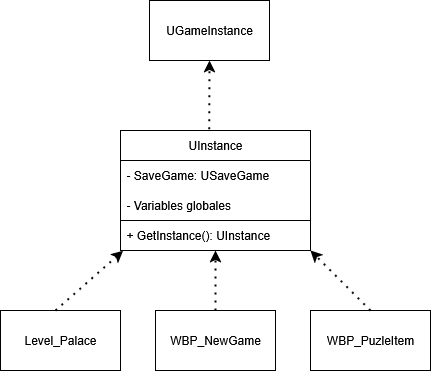
\includegraphics[width=\textwidth]{../img/anexos/ejemplo_singleton.png}
	\label{b:ejemplo_singleton}
\end{figure}

\subsection{Patrón \textit{Command}}

El patrón de diseño \textit{Command} se aplica para gestionar acciones que deben ejecutarse como respuesta a condiciones específicas del entorno de juego, manteniendo bajo acoplamiento entre los objetos emisores y receptores.

Este patrón encapsula una petición (acción) como un objeto, permitiendo su almacenamiento, programación o ejecución diferida. En Unreal Engine, esta lógica se implementa comúnmente mediante \textit{event dispatchers} o \textit{delegates}, herramientas que permiten vincular eventos con funciones de manera flexible.

Ejemplos concretos en el proyecto:
\begin{itemize}
    \item \textbf{Evento de apertura de caja:} Cuando todos los candados están resueltos, se emite un evento que ejecuta la animación de apertura de la caja. El objeto ``candado`` no necesita conocer directamente la lógica interna de la caja, sólo invocar el comando asociado.
    
    \item \textbf{Evento de finalización del juego:} Al cumplirse los criterios de éxito de la tarea motriz, se lanza un comando que activa la animación final, la recolección de métricas y la transición de nivel. Todo ello está encapsulado en un conjunto de acciones invocadas como comandos.
\end{itemize}

\textbf{Ventajas en el contexto del proyecto:}
\begin{itemize}
    \item Desacopla la lógica de condición (candado, éxito, tiempo, etc.) de la lógica de ejecución.
    \item Permite reutilizar, programar o modificar comandos sin afectar el código fuente de los objetos emisores.
    \item Facilita la modularidad y mantenimiento del sistema VR, donde múltiples interacciones generan eventos secuenciados.
\end{itemize}

\begin{figure}[h]
	\caption[Ejemplo de command]{Ejemplo del patrón \textit{command} en el proyecto.}
	\centering
	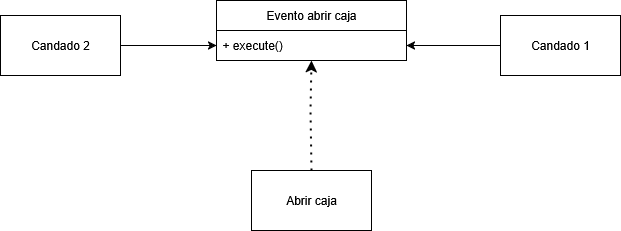
\includegraphics[width=\textwidth]{../img/anexos/ejemplo_patron_command.png}
	\label{b:ejemplo_command}
\end{figure}


\subsection*{Despliegue}

La aplicación está diseñada para ejecutarse como una aplicación de escritorio en sistemas operativos Windows. El entorno de realidad virtual se experimenta a través del visor \textit{Meta Quest 2}, utilizando la funcionalidad \textit{Meta Quest Link}, que permite al dispositivo actuar como pantalla y controlador de entrada para el equipo principal.

El proceso de despliegue y ejecución sigue los siguientes pasos:

\begin{enumerate}
  \item El proyecto se compila en \texttt{Unreal Engine 5} en formato ejecutable \texttt{.exe} para Windows, utilizando el modo \texttt{VR Preview} para pruebas o el empaquetado estándar para distribución.
  \item El visor \textit{Meta Quest 2} se conecta al ordenador mediante cable USB o por conexión inalámbrica compatible (\textit{Air Link}), utilizando la funcionalidad \textit{Meta Quest Link} para emular una pantalla secundaria en realidad virtual.
  \item Al ejecutar la aplicación en el equipo, el usuario puede visualizar e interactuar con el entorno virtual desde el visor, con seguimiento completo de movimiento y controladores hápticos.
\end{enumerate}

Este enfoque de despliegue permite aprovechar toda la potencia gráfica del equipo de desarrollo, eliminando las limitaciones de hardware del visor autónomo. Además, facilita el desarrollo iterativo, la depuración en tiempo real y el uso de recursos más exigentes sin afectar al rendimiento.

\section{Diseño procedimental}

En el desarrollo de \textit{software}, el diseño procedimental hace referencia a la definición estructurada y detallada de los pasos necesarios para llevar a cabo funcionalidades concretas dentro de la aplicación. Este enfoque se basa en la descomposición del problema en tareas elementales y secuenciales que, en conjunto, permiten alcanzar un objetivo funcional específico.

En el presente proyecto, el diseño procedimental se ha representado mediante diagramas de secuencia siguiendo la notación de \textit{UML 2}. Estos diagramas permiten visualizar la interacción entre los distintos componentes del sistema —clases, \textit{blueprints}, interfaces de usuario y controladores de entorno— durante la ejecución de los distintos procesos clave de la aplicación.

A continuación, se muestran los diagramas correspondientes a algunas de las funcionalidades principales del sistema, como el proceso de guardado de estado, la carga de partidas, o la gestión de eventos dentro de los puzles, con el objetivo de facilitar la comprensión de su comportamiento dinámico.

\subsection{Registro}
En el diagrama de secuencia \ref{fig:diagrama_secuencia_registro} se muestran los pasos que sigue el programa al registrarse por primera vez:
\begin{figure}[H]
    \centering
    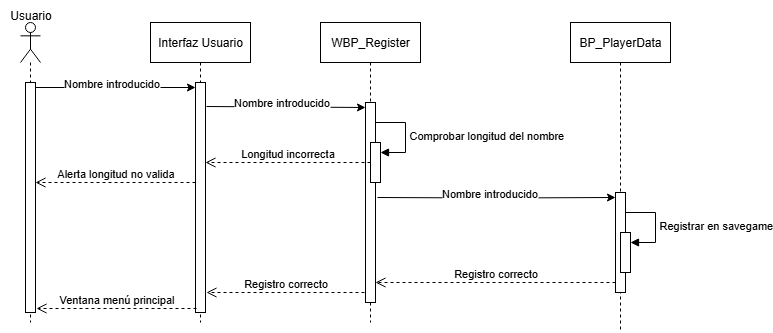
\includegraphics[width=\textwidth]{../img/anexos/diagrama_secuencia_registro.png}
    \caption[Diagrama de secuencia de registro]{Diagrama de secuencia del registro por primera vez}
    \label{fig:diagrama_secuencia_registro}
\end{figure}

\subsection{Crear nueva partida}
En el diagrama de secuencia \ref{fig:diagrama_secuencia_nuevopuzle} se muestran los pasos que sigue el programa al crear un nuevo puzle.
\begin{figure}[H]
    \centering
    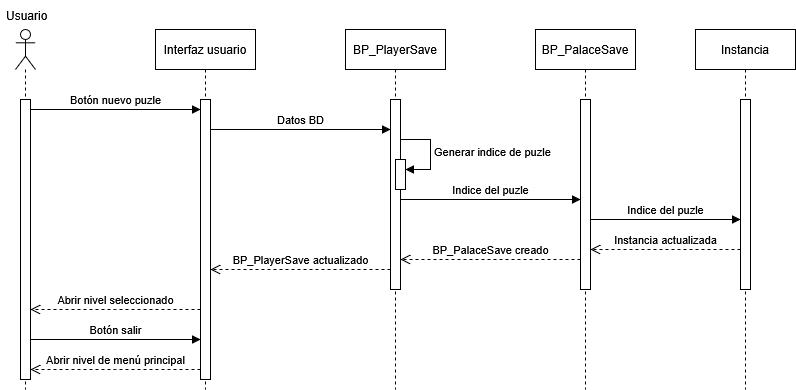
\includegraphics[width=\textwidth]{../img/anexos/diagrama_secuencia_nuevopuzle.png}
    \caption[Diagrama de secuencia de nueva partida]{Diagrama de secuencia de nueva partida}
    \label{fig:diagrama_secuencia_nuevopuzle}
\end{figure}

\subsection{Cargado de partida}
En el diagrama de secuencia \ref{fig:diagrama_secuencia_cargado} se muestran los pasos que sigue el programa para cargar un puzle.

\begin{figure}[H]
    \centering
    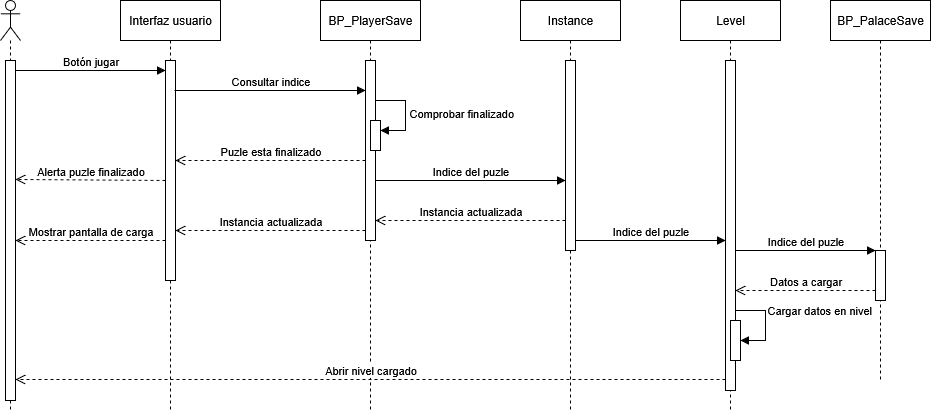
\includegraphics[scale=0.40]{../img/anexos/diagrama_secuencia_carga.png}
    \caption[Diagrama de secuencia cargado de partida]{Diagrama de secuencia de cargado de partida}
    \label{fig:diagrama_secuencia_cargado}
\end{figure}
\apendice{Documentación técnica de programación}

\section{Introducción}

\section{Estructura de directorios}

\section{Manual del programador}

\section{Compilación, instalación y ejecución del proyecto}

\section{Pruebas del sistema}

\apendice{Documentación de usuario}

\section{Introducción}

\section{Requisitos de usuarios}

\section{Instalación}

\section{Manual del usuario}



\apendice{Anexo de sostenibilización curricular}

\section{Introducción}
Este anexo incluirá una reflexión personal del alumnado sobre los aspectos de la sostenibilidad que se abordan en el trabajo.
Se pueden incluir tantas subsecciones como sean necesarias con la intención de explicar las competencias de sostenibilidad adquiridas durante el alumnado y aplicadas al Trabajo de Fin de Grado.

Más información en el documento de la CRUE \url{https://www.crue.org/wp-content/uploads/2020/02/Directrices_Sosteniblidad_Crue2012.pdf}.

Este anexo tendrá una extensión comprendida entre 600 y 800 palabras.



\bibliographystyle{plain}
\bibliography{bibliografiaAnexos}

\end{document}
